\subsection{Abstract Factory}
	\begin{figure}[h!]
	\begin{center}
		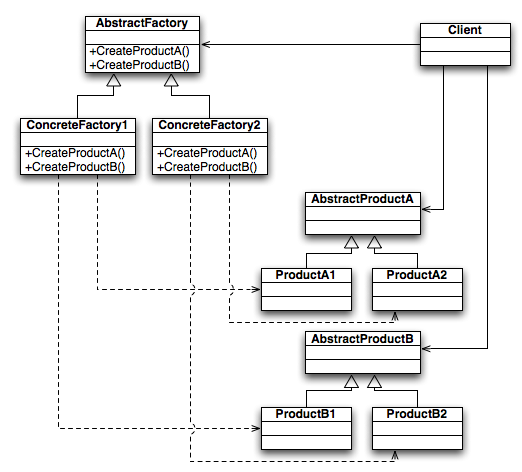
\includegraphics[scale=1]{../images/AbsFactory.png}
		\caption{Design Pattern Abstract Factory}
	\end{center}
	\end{figure}
	\begin{itemize}
		\item\textbf{Scopo}: fornire al Client un'interfaccia per creare famiglie di prodotti, senza dover esplicitare il nome concreto delle classi a cui si riferisce. La factory, quindi, incapsula le responsabilità per la creazione degli oggetti prodotto.
		\item\textbf{Applicabilità}:
		\begin{itemize}
			\item quando si necessita di rendere indipendente un sistema dalla creazione dei suoi componenti, dalla loro rappresentazione e composizione.
			\item quando si necessita la configurazione di un sistema scegliendo tra più tipologie.
			\item quando si devono gestire famiglie di prodotti correlati tra loro e progettati per essere usati insieme.
			\item quando si vuole rivelare solamente l'interfaccia delle classi all'interno di una libreria.
		\end{itemize}
		\item\textbf{Conseguenze}:
		\begin{itemize}
			\item isola le classi concrete, controllandone la creazione. La creazione è delegata
alla classe astratta e i Client manipolano solamente interfacce non conoscendo
i nomi dei prodotti nascosti
			\item permette di modificare facilmente la famiglia di prodotti utilizzati poiché la
classe concreta appare una sola volta nel programma
			\item promuove la coerenza nell'utilizzo dei prodotti poiché sono stati progettati per
essere utilizzati insieme (si usano oggetti di una sola famiglia per volta)
			\item risulta invece difficile l'inserimento di nuove tipologie di prodotto poichè richiederebbe la modifica della classe di Abstract Factory e di conseguentemente il
cambiamento di tutte le sottoclassi (il problema può essere evitato mediante
una tecnica di implementazione della classe astratta, ma in modo meno flessibile e poco sicuro.
		\end{itemize}
		\item\textbf{Utilizzo}: nel sistema Quizzipedia il design pattern è stato utilizzato nel package Interpreter. Il package si avvale del pattern per rendere il sistema indipendente dalla creazione delle classi concrete ed essere aperto all'estensione tramite la definizione di nuovi tipi "Interpreter".

	\begin{figure}[h!]
	\begin{center}
		\includegraphics[scale=0.5]{../images/interpreterClass.png}
		\caption{Abstract Factory in Interpreter}
	\end{center}
	\end{figure}
	\end{itemize}
	
	\subsection{Singleton}
	\begin{figure}[h!]
	\begin{center}
		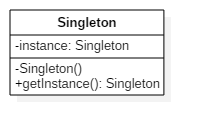
\includegraphics[scale=0.7]{../images/Singleton.png}
		\caption{Design Pattern Singleton}
	\end{center}
	\end{figure}
	\begin{itemize}
		\item\textbf{Scopo}: assicurare l'esistenza di una sola istanza di un oggetto, offrendo un punto globale di accesso a tale istanza.
		\item\textbf{Applicabilità}:
		\begin{itemize}
			\item quando deve essere creata una sola istanza di una classe e deve esistere un punto di accesso ad essa noto a tutti Client
			\item quando l'istanza deve poter essere estesa e i Client devono essere in grado di
utilizzarne le istanze senza apportare modifiche al proprio codice
		\end{itemize}
		\item\textbf{Conseguenze}:
		\begin{itemize}
			\item l'accesso all'unica istanza è controllato
			\item permette di aver un miglior uso delle variabili globali, riducendo lo spazio dei nomi senza inquinarlo con variabili utilizzate per memorizzare riferimenti ad
istanze
			\item maggior  flessibilità per quanto riguarda le operazioni di classe, ma maggior
difficoltà nelle modifiche del progetto per utilizzare più istanze. Impossibilità
di sovrascrivere le funzioni di classe poiché statiche e non virtuali.
		\end{itemize}
		\item\textbf{Utilizzo}: nel sistema Quizzipedia il design pattern è stato utilizzato per le classi\\
		 QML2HTMLQuestionFactory e QMLInterpreterFactory. Usato in collaborazione con\\ l'\emph{Abstract Factory}, il pattern assicura che la costruzione degli oggetti Interpreter e Question abbia un unico punto d'accesso nelle classi sopracitate.
	\end{itemize}		
	
	\subsection{Publish - Subscribe}
	\begin{figure}[h!]
	\begin{center}
		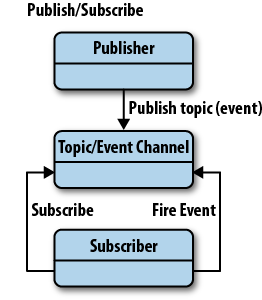
\includegraphics[scale=1.2]{../images/publish-subscribe-pattern.png}
		\caption{Design Pattern Publish-Subscribe}
	\end{center}
	\end{figure}
	\begin{itemize}
		\item\textbf{Scopo}: in questo schema, mittenti e destinatari di messaggi dialogano attraverso un tramite, che può essere detto dispatcher o broker. Il mittente di un messaggio (detto publisher) non deve essere consapevole dell'identità dei destinatari (detti subscriber); esso si limita a "pubblicare" (in inglese to publish) il proprio messaggio al dispatcher. I destinatari si rivolgono a loro volta al dispatcher "abbonandosi" (in inglese to subscribe) alla ricezione di messaggi. Il dispatcher quindi inoltra ogni messaggio inviato da un publisher a tutti i subscriber interessati a quel messaggio.
		\item\textbf{Applicabilità}:
		\begin{itemize}
			\item implementare la comunicazione asincrona tra diverse componenti
			\item rendere disponibili al Client solo una parte ristretta dei dati d'interesse.
		\end{itemize}
		\item\textbf{Conseguenze}:
		\begin{itemize}
			\item disaccoppiamento tra publisher e subscribers
			\item alta scalabilità
			\item scarsa flessibilità nella struttura dei dati pubblicati.
		\end{itemize}
		\item\textbf{Utilizzo}: nel sistema Quizzipedia il design pattern è stato utilizzato per le classi Publishers e Subscribers, il cui funzionamento è del tutto analogo a quanto descritto sopra. Va notato che nel framework Meteor la componente 'dispatcher' è completamente trasparente al programmatore. E' sufficiente 'pubblicare' i dati lato server e 'abbonarsi' ai dati lato client, Meteor si preoccuperà della comunicazione client-server.
		
	\begin{figure}[h!]
	\begin{center}
		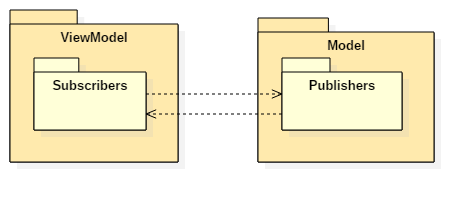
\includegraphics[scale=0.8]{../images/PublishSubscribeDesignPattern.png}
		\caption{Publish-Subscribe in Quizzipedia}
	\end{center}
	\end{figure}
	\end{itemize}
	\newpage